% answers.tex —— 1956 年·全国卷 · 参考答案与详细解析片段
% 由 tools/generate_projects.py 依来源总账自 1956/1956_数学真题_试题.md + 1956/1956_数学真题_解析正文.md + 1956/1956_数学真题_答案要点.md 生成，勿手改（改源 MD 后重跑）


\gkpart{一、小题}

\begin{answer}
\gksolhead{1}{}

\textbf{题目}：

（甲）利用对数性质，计算 $(\lg 5)^2+\lg 2\cdot\lg 50$。

（注：原卷中第一个 2 为上标，表示 $(\lg 5)^2$。）

\Needspace{4\baselineskip}
\textbf{解析}

令 $a=\lg5$。由于 $\lg2+\lg5=1$，有 $\lg2=1-a$；又 $\lg50=\lg(2\cdot25)=\lg2+2\lg5=1+a$。因此
\[
(\lg5)^2+\lg2\cdot\lg50
=a^2+(1-a)(1+a)
=a^2+1-a^2=1.
\]

\gkanswer{答案：$1$}

\end{answer}
\begin{answer}
\gksolhead{2}{}

\textbf{题目}：

（乙）设 $m$ 是实数，求证方程
\[
2x^2-(4m-1)x-m^2-m=0
\]
的两个根必定都是实数。

\Needspace{4\baselineskip}
\textbf{解析}

方程为 $2x^2-(4m-1)x-m^2-m=0$，其判别式为
\[
\Delta=[-(4m-1)]^2-4\cdot2\cdot(-m^2-m)
=(4m-1)^2+8m^2+8m
=24m^2+1.
\]
因 $m\in\mathbf R$，故 $m^2\geqslant0$，从而 $\Delta>0$。所以方程有两个不相等的实根。

\gkanswer{答案：对任意实数 $m$，方程有两个不相等的实根。}

\end{answer}
\begin{answer}
\gksolhead{3}{}

\textbf{题目}：

（丙）设 $M$ 是 $\triangle ABC$ 的边 $AC$ 的中点，过 $M$ 作直线交 $AB$ 直线于 $E$，过 $B$ 作直线平行于 $ME$ 交 $AC$ 直线于 $F$。求证 $\triangle AEF$ 的面积等于 $\triangle ABC$ 的面积的一半。

\Needspace{4\baselineskip}
\textbf{解析}
\nopagebreak[4]
\begin{center}% 1956 年全国卷第 7 题：等边三角形外接圆上的点 P 与 AP、BC 交点 M。
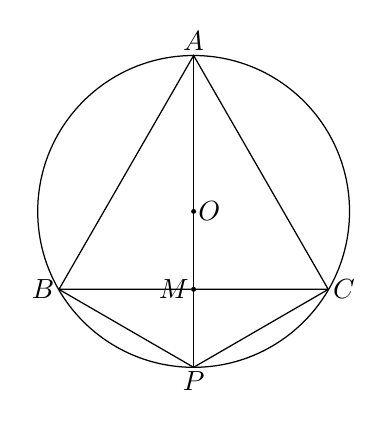
\begin{tikzpicture}[scale=0.9, line width=0.45pt,
  every node/.style={inner sep=1.5pt}]
  \coordinate (O) at (0,0);
  \coordinate (A) at (0,2.2);
  \coordinate (B) at (-1.9,-1.1);
  \coordinate (C) at (1.9,-1.1);
  \coordinate (P) at (0,-2.2);
  \coordinate (M) at (0,-1.1);
  \draw (O) circle (2.2);
  \draw (A)--(B)--(C)--cycle;
  \draw (A)--(P);
  \draw (B)--(P)--(C);
  \draw (B)--(C);
  \fill (O) circle (0.035) (M) circle (0.035);
  \node[anchor=south] at (A) {$A$};
  \node[anchor=east] at (B) {$B$};
  \node[anchor=west] at (C) {$C$};
  \node[anchor=north] at (P) {$P$};
  \node[anchor=west] at (O) {$O$};
  \node[anchor=east] at (M) {$M$};
\end{tikzpicture}
\end{center}
\nopagebreak[4]
在 $\triangle ABC$ 中，$M$ 是 $AC$ 的中点，$E$ 在 $AB$ 所在直线上，$F$ 在 $AC$ 所在直线上，且 $BF\parallel ME$。由平行线可得
\[
\triangle ABF\sim\triangle AEM,
\qquad \frac{AB}{AE}=\frac{AF}{AM}.
\]
三角形 $AEF$ 与 $ABC$ 的两边分别落在同两条直线 $AB$、$AC$ 上，故
\[
\frac{S_{\triangle AEF}}{S_{\triangle ABC}}
=\frac{AE}{AB}\cdot\frac{AF}{AC}
=\frac{AE}{AB}\cdot\frac{AF}{AM}\cdot\frac{AM}{AC}
=1\cdot\frac12=\frac12.
\]
因此 $S_{\triangle AEF}=\dfrac12S_{\triangle ABC}$。当 $E$ 位于 $AB$ 的延长线上时，上式按有向线段理解，取普通面积后结论不变。

\gkanswer{答案：$S_{\triangle AEF}=\dfrac12S_{\triangle ABC}$。}

\end{answer}
\begin{answer}
\gksolhead{4}{}

\textbf{题目}：

（丁）一个三角形三边的长分别是 $3$ 尺、$4$ 尺及 $\sqrt{37}$ 尺，求这个三角形的最大角的度数。

\Needspace{4\baselineskip}
\textbf{解析}

最大角与最大边相对。设边 $\sqrt{37}$ 所对的角为 $\theta$，由余弦定理
\[
37=3^2+4^2-2\cdot3\cdot4\cos\theta.
\]
所以
\[
\cos\theta=\frac{9+16-37}{24}=-\frac12,
\qquad \theta=120^\circ.
\]

\gkanswer{答案：$120^\circ$。}

\end{answer}
\begin{answer}
\gksolhead{5}{}

\textbf{题目}：

（戊）设 $\tan\alpha$ 与 $\tan\beta$ 是方程 $x^2+6x+7=0$ 的两个根，求证
\[
\sin(\alpha+\beta)=\cos(\alpha+\beta).
\]

\Needspace{4\baselineskip}
\textbf{解析}

令 $u=\tan\alpha$，$v=\tan\beta$。由韦达定理
\[
u+v=-6,\qquad uv=7.
\]
于是
\[
\tan(\alpha+\beta)=\frac{u+v}{1-uv}=\frac{-6}{1-7}=1.
\]
因 $1-uv=-6\neq0$，正切加法公式合法，故 $\sin(\alpha+\beta)=\cos(\alpha+\beta)$。

\gkanswer{答案：$\sin(\alpha+\beta)=\cos(\alpha+\beta)$。}

\end{answer}
\gkpart{二、大题}

\begin{answer}
\gksolhead{6}{}

\textbf{题目}：

解联立方程
\[
\begin{cases}
7\sqrt{x+y}-x-y=12,\\
x^2+y^2=136.
\end{cases}
\]

\Needspace{4\baselineskip}
\textbf{解析}

令 $s=x+y$，$t=\sqrt{s}$，则 $t\geqslant0$，第一式化为
\[
7t-t^2=12,
\qquad (t-3)(t-4)=0.
\]
所以 $s=9$ 或 $s=16$。

当 $s=9$ 时，
\[
(x-y)^2=2(x^2+y^2)-(x+y)^2=272-81=191,
\]
故 $x-y=\pm\sqrt{191}$，得到
\[
(x,y)=\left(\frac{9+\sqrt{191}}2,\frac{9-\sqrt{191}}2\right),
\quad
\left(\frac{9-\sqrt{191}}2,\frac{9+\sqrt{191}}2\right).
\]

当 $s=16$ 时，
\[
(x-y)^2=272-256=16,
\]
故 $x-y=\pm4$，得到 $(x,y)=(10,6)$ 或 $(6,10)$。代回原方程组，四组解均成立。

\gkanswer{答案：$(x,y)=\left(\frac{9+\sqrt{191}}2,\frac{9-\sqrt{191}}2\right),\ \left(\frac{9-\sqrt{191}}2,\frac{9+\sqrt{191}}2\right),\ (10,6),\ (6,10)$}

\end{answer}
\begin{answer}
\gksolhead{7}{}

\textbf{题目}：

设 $P$ 是等边三角形 $ABC$ 外接圆不含 $A$ 的小弧 $\widehat{BC}$ 上的一点，求证
\[
PA^2=AB^2+PB\cdot PC.
\]

\Needspace{4\baselineskip}
\textbf{解析}

设 $M=AP\cap BC$。由于 $P$ 位于外接圆不含 $A$ 的小弧 $BC$ 上，由圆周角定理和等边三角形性质，
\[
\angle APB=\angle ACB=60^\circ=\angle ABM,
\]
且 $\angle BAP=\angle BAM$。因此 $\triangle ABP\sim\triangle AMB$，从而
\[
AP\cdot AM=AB^2.\tag{1}
\]
另一方面，$A,M,P$ 共线、$B,M,C$ 共线，故
\[
\angle APC=\angle BPM,\qquad \angle PAC=\angle PBM.
\]
于是 $\triangle ACP\sim\triangle BMP$，得到
\[
AP\cdot MP=PB\cdot PC.\tag{2}
\]
将（1）、（2）相加，并利用 $AM+MP=AP$，得
\[
AP^2=AP(AM+MP)=AB^2+PB\cdot PC.
\]

\gkanswer{答案：$PA^2=AB^2+PB\cdot PC$}

\end{answer}
\begin{answer}
\gksolhead{8}{}

\textbf{题目}：

有一四棱柱体，底面 $ABCD$ 为菱形，且
$\angle A'AB=\angle A'AD$（如图），求证平面 $A'ACC'$ 垂直于底面 $ABCD$。
\nopagebreak[4]
\begin{center}% 1956 年全国卷第 8 题：底面 ABCD 为菱形的四棱柱示意图。
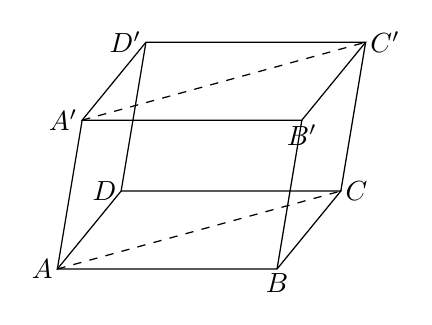
\begin{tikzpicture}[scale=0.9, line width=0.45pt,
  every node/.style={inner sep=1.5pt}]
  \coordinate (A) at (0,0);
  \coordinate (B) at (3.1,0);
  \coordinate (C) at (4.0,1.1);
  \coordinate (D) at (0.9,1.1);
  \coordinate (A1) at (0.35,2.1);
  \coordinate (B1) at (3.45,2.1);
  \coordinate (C1) at (4.35,3.2);
  \coordinate (D1) at (1.25,3.2);
  \draw (A)--(B)--(C)--(D)--cycle;
  \draw (A1)--(B1)--(C1)--(D1)--cycle;
  \draw (A)--(A1) (B)--(B1) (C)--(C1) (D)--(D1);
  \draw[dashed] (A)--(C) (A1)--(C1);
  \node[anchor=east] at (A) {$A$};
  \node[anchor=north] at (B) {$B$};
  \node[anchor=west] at (C) {$C$};
  \node[anchor=east] at (D) {$D$};
  \node[anchor=east] at (A1) {$A'$};
  \node[anchor=north] at (B1) {$B'$};
  \node[anchor=west] at (C1) {$C'$};
  \node[anchor=east] at (D1) {$D'$};
\end{tikzpicture}
\end{center}
\nopagebreak[4]
\Needspace{4\baselineskip}
\textbf{解析}
\nopagebreak[4]
\begin{center}% 1956 年全国卷第 8 题解析图：加入 AC、BD、交点 O 与 A'O。
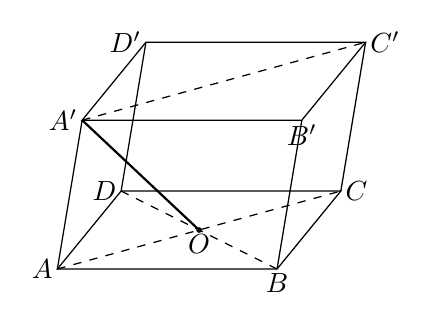
\begin{tikzpicture}[scale=0.9, line width=0.45pt,
  every node/.style={inner sep=1.5pt}]
  \coordinate (A) at (0,0);
  \coordinate (B) at (3.1,0);
  \coordinate (C) at (4.0,1.1);
  \coordinate (D) at (0.9,1.1);
  \coordinate (A1) at (0.35,2.1);
  \coordinate (B1) at (3.45,2.1);
  \coordinate (C1) at (4.35,3.2);
  \coordinate (D1) at (1.25,3.2);
  \coordinate (O) at (2.0,0.55);
  \draw (A)--(B)--(C)--(D)--cycle;
  \draw (A1)--(B1)--(C1)--(D1)--cycle;
  \draw (A)--(A1) (B)--(B1) (C)--(C1) (D)--(D1);
  \draw[dashed] (A)--(C) (B)--(D) (A1)--(C1);
  \draw[thick] (A1)--(O);
  \fill (O) circle (0.04);
  \node[anchor=east] at (A) {$A$};
  \node[anchor=north] at (B) {$B$};
  \node[anchor=west] at (C) {$C$};
  \node[anchor=east] at (D) {$D$};
  \node[anchor=east] at (A1) {$A'$};
  \node[anchor=north] at (B1) {$B'$};
  \node[anchor=west] at (C1) {$C'$};
  \node[anchor=east] at (D1) {$D'$};
  \node[anchor=north] at (O) {$O$};
\end{tikzpicture}
\end{center}
\nopagebreak[4]
设 $O$ 为菱形两条对角线 $AC$、$BD$ 的交点。菱形的对角线互相垂直且互相平分，所以 $AO\perp BD$，且 $O$ 是 $BD$ 的中点。

在 $\triangle A'AB$ 与 $\triangle A'AD$ 中，$AA'$ 为公共边，$AB=AD$，且题设给出 $\angle A'AB=\angle A'AD$。由边角边，
\[
\triangle A'AB\cong\triangle A'AD,
\]
所以 $A'B=A'D$。因此 $\triangle A'BD$ 为等腰三角形，$O$ 是其底边 $BD$ 的中点，故 $A'O\perp BD$。

直线 $AO$、$A'O$ 是平面 $A'OA$ 内相交的两条直线，且均垂直于 $BD$，所以 $BD\perp$ 平面 $A'OA$。又因 $A'C'\parallel AC$，平面 $A'OA$ 即平面 $A'ACC'$。故该平面垂直于底面 $ABCD$。

\gkanswer{答案：平面 $A'ACC'$ 垂直于底面 $ABCD$}

\end{answer}
\begin{answer}
\gksolhead{9}{}

\textbf{题目}：

若三角形的三个角成等差级数，则其中一定有一个角是 $60^\circ$；试证明之。

\Needspace{4\baselineskip}
\textbf{解析}

将三个角按从大到小排列为 $A$、$B$、$C$。因三角形内角成等差级数，
\[
A-B=B-C,\qquad A+B+C=180^\circ.
\]
写成 $A=B+d$、$C=B-d$ 后相加，得 $3B=180^\circ$，即 $B=60^\circ$。所以三个角中必有一个是 $60^\circ$。

\gkanswer{答案：三个角中间的一个为 $60^\circ$，所以必有一个角是 $60^\circ$}

\end{answer}
\begin{answer}
\gksolhead{10}{}

\textbf{题目}：

若上述三角形的三边又成等比级数，则三个角都是 $60^\circ$，试证明之。

\Needspace{4\baselineskip}
\textbf{解析}

在第 9 题条件下，将三边按从小到大排列为 $a$、$aq$、$aq^2$，其中 $a>0$、$q\geqslant1$。边和角按大小对应，因此中间边 $aq$ 所对的角为 $60^\circ$。由余弦定理
\[
(aq)^2=a^2+(aq^2)^2-2\cdot a\cdot aq^2\cos60^\circ.
\]
代入 $\cos60^\circ=\dfrac12$ 并除以 $a^2$，得
\[
q^2=1+q^4-q^2,
\qquad (q^2-1)^2=0.
\]
因 $q\geqslant1$，故 $q=1$。三边相等，三角形为等边三角形，三个角都是 $60^\circ$。

\gkanswer{答案：三边相等，故三个角都是 $60^\circ$}

\end{answer}